\documentclass[a4paper]{article}
\usepackage{graphicx}
\usepackage{enumitem}
\usepackage[top=0.9in, bottom=1in]{geometry}

\title{Massive Data Analysis - Similarity in Book Reviews - Using MinHashLSH and Jaccard Algorithm}
\author{Akash Mittal (31909A) | Antonella Convertini (45853A)}
\date{\today}

\maketitle

\begin{abstract}
The project explores and investigates the similarity between book reviews using Jaccard Similarity. We have implemented MinHash Locality Sensitive Hashing (LSH) on a different sampled subset of Amazon book reviews and made the code scalable to run on large dataset. The objective is to identify similar reviews efficiently at scale, so we used Spark for distributed processing. Further, we focussed on similar reviews by filtering out various stop words and filler text.
\end{abstract}

\section{Introduction}
Finding similar reviews in a large corpus is a fundamental problem in NLP and recommender systems. Traditional Jaccard similarity becomes computationally expensive for large datasets, so we explore approximate methods like MinHashLSH to scale similarity detection. Spark is used for its ability to handle large datasets in parallel.

\section{Dataset}
The dataset used is \textbf{Amazon Book Reviews}, containing 3 million reviews. We used the \texttt{Books\_rating.csv} file which includes fields such as:
\begin{itemize}
  \item \texttt{'Id'}
  \item \texttt{'Title'}
  \item \texttt{'Price'}
  \item \texttt{'User_id'}
  \item \texttt{'profileName'}
  \item \texttt{'review/helpfulness'}
  \item \texttt{'review/score'}
  \item \texttt{'review/time'}
  \item \texttt{'review/summary'}
  \item \texttt{'review/text'}
\end{itemize}

\vspace{-\baselineskip}
\pagebreak

Due to computation constraints, we processed random samples of the data but used a seed to keep the outputs reproducible. 
Further, we used only IDs and review text to find similar pairs. 
Additionally, we created a unique \texttt{review\_id} for each review using the fields \texttt{'Id'}, \texttt{'User\_id'}, and \texttt{'review/time'}.

\section{Preprocessing}
\begin{itemize}
  \item We removed null and  very short reviews <25 length of characters (it can be configured using \texttt{REVIEW\_LENGTH} threshold).
  \item We tokenized and cleaned the review text.
  \item On the tokenized dataset, we applied lemmatization using NLTK.
  \item From the structured lemmatized tokens we removed stopwords.
  \item From the lemmatized tokens, we removed stopwords. These stopwords were imported from NLTK and combined with the following custom stopwords:
  \begin{itemize}
    \item\texttt{\{"book", "read", "word", "paragraph", "magazine", "novel", "page", "chapter"\}}
  \end{itemize}
  \item Then, we filtered the tokens by length (\texttt{TOKEN\_SIZE} = 5), and it removes the review for which we have less than 5 tokens.
\end{itemize}

\section{Methodology}

We used the following steps on the lemmatized tokens to compute similarity between the reviews:

\subsection*{1. Token Vectorization}
We used Spark's \texttt{Tokenizer} and \texttt{HashingTF} to convert cleaned and lemmatized tokens into feature vectors.

\subsection*{2. Approximate Jaccard Similarity}
We used \texttt{MinHashLSH} from Spark MLlib library:
\begin{itemize}
  \item Trained on hashed token vectors.
  \item Computed pairwise approximate Jaccard similarities.
  \item Filtered pairs using a threshold (Jaccard Distance $< 0.6$), thus Jaccard Similarity >= 0.4 (40%)
\end{itemize}


\section{Results}

The similarity computation was done for a different sampled fractions of the dataset. 
The results and insights from each are as follows :

\begin{table}[h!]
    \centering
    \caption{Performance metrics and similarity results across different dataset sample sizes.}
    \begin{tabular}{lcccc}
        \toprule
        \textbf{Metric} & \textbf{0.5\%} & \textbf{0.75\%} & \textbf{1\%} & \textbf{2\%} \\
        \midrule
        Sampled Reviews & 15,189 & 22,779 & 30,332 & 60,498 \\
        Filtered Sampled Reviews & 15,013 & 22,442 & 29,808 & 58,797 \\
        Sampling Time (min) & 0.02 & 0.80 & 0.80 & 0.81 \\
        Filtering Time (min) & 0.15 & 0.11 & 0.09 & 0.14 \\
        Text Processing Time (min) & 0.01 & 0.01 & 0.01 & 0.01 \\
        Hashing Time (min) & 5.08 & 5.15 & 5.32 & 5.93 \\
        LSH Time (min) & 0.06 & 0.10 & 0.09 & 0.07 \\
        Jaccard Time (min) & 3.74 & 7.69 & 14.77 & 50.45 \\
        Similar Pairs Found & 9 & 17 & 30 & 135 \\
        \bottomrule
    \end{tabular}
\end{table}

From the above analysis, we see that the processing steps are run with consistent time limits for different steps, thus they are scaling well with the increased dataset.
However, the "Jaccard Similarity" step shows a steep and non-linear increase in runtime as the sample fraction grows, which is due to the fact the pairwise similarity becomes expensive with increased number of candidate pairs.

\section{Analysis of Similar Pairs found in 2\% sampled fraction of Dataset}

\begin{itemize}
    \item We found \textbf{135} similar pairs in the \textbf{2\%} sampled dataset for \textbf{>= 40\%} similarity. Further, we observed that many pairs were almost identical even after we removed the duplicates. This is due to the fact of various typos in text, some additional filler words in reviews and slight variation of reviews posted under different books etc.
        
        \item We counted review pairs with exact (\textbf{>95\%})and near exact matches of the reviews. 
        
        \begin{table}
            \begin{tabular}{cc}
                 Match Type& Count\\
                 Exact Match& 4\\
                 Near Match& 131\\
            \end{tabular}
        \end{table}
\item From the review pairs, we calculated the unique book counts to be \textbf{199} based on the "bookid".
\item Below is a plot for Jaccard Distances Distribution for the Review Pairs :

\begin{figure}
    \centering
    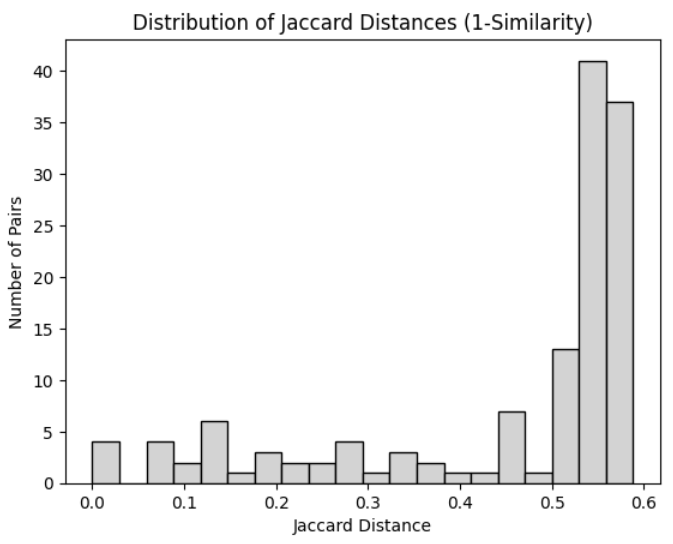
\includegraphics[width=0.5\linewidth]{Jaccard_Distance_Distribution.png}
    \caption{Distribution of Jaccard Distance}
    \label{Fig. 1}
\end{figure}

\item Then we calculated that there are \textbf{17} book review pairs with almost identical reviews but different book IDs.
\begin{itemize}
    \item These different book ids with the same reviews introduces suspicion and also points out to plagiarism in reviews. It also points out that there can be different bookid for same book which are present in the dataset. And the reveiws just show redundant data (maybe sourced from different platforms), if not plagiarised.  
So we analyzed the pairs where bookids are different but reviews are similar (to filter out similar reviews for same books)  
\end{itemize}

\item The count of review pairs where reviews are similar for different books, is \textbf{131} (out of 135) (based on book ids only). Thus, almost all review pairs have different books (or can have same book if it is mentioned with different id for different reasons, e.g. version of book) .
    
    \item The below plot shows the distribution of similar books reviews frequency:
    \begin{figure}
        \centering
        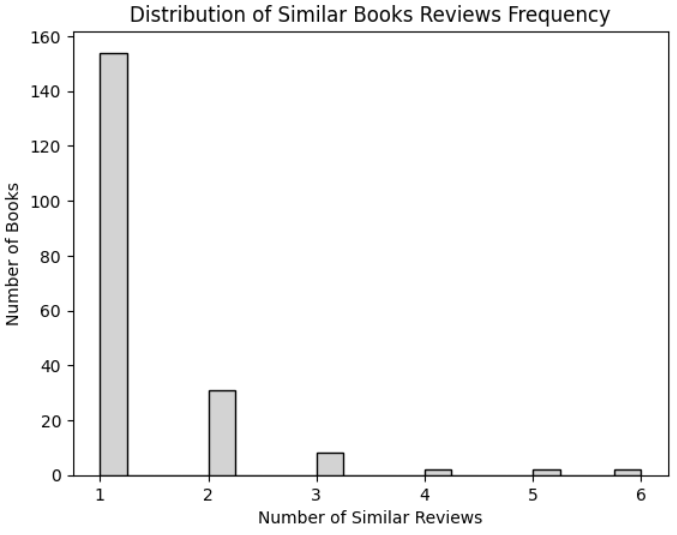
\includegraphics[width=0.5\linewidth]{Distribution of Similar Books Reviews Frequency.png}
        \caption{Distribution of Similar Books Reviews Frequency}
        \label{Fig. 2}
    \end{figure}

    \item Finally, we created a wordcloud for words in reviews column from the \textbf{135 }similar books:
    
\begin{figure}
    \centering
    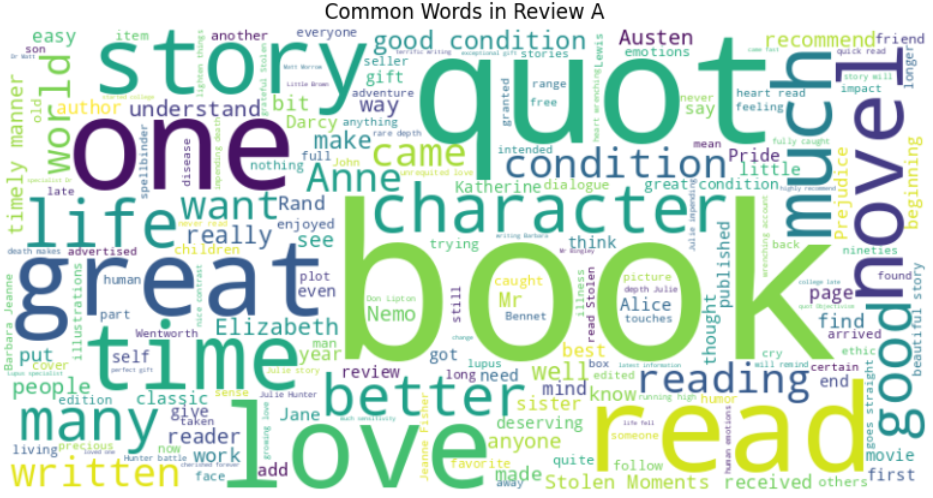
\includegraphics[width=1\linewidth]{WordCloud_Similar_Pairs.png}
    \caption{WordCloud}
    \label{Fig. 3}
\end{figure}
\end{itemize}

\section{Limitations}
\begin{itemize}
  \item We compute only the approximate similarity from similar candidate pairs using LSH, and didn't compare whole dataset which will cost O(N*N) complexity.
  \item Since we are using Jaccard Similarity, there is no semantic meaning capture.
  \item Since, we also removed the stopwords and other common words along with limiting the review length and token length, we are not accounting in short reviews that may be just like {'I loved this book, always recommend", "The book is very nice to read" etc. } 
\end{itemize}

\section{Conclusion}
This project explains how \textbf{MinHashLSH} can be used to efficiently compute review similarities in a large dataset. Further, we also highlight that how computationally the algorithms become when running on massive datasets, which calls for optimized algorithms that pulls in a trade-off between precision and recall of the desired objective (similarity analysis in our case).

\section{Declaration}

\textit{“We declare that this material, which we now submit for assessment, is entirely our own work and has not been taken from the work of others, save and to the extent that such work has been cited and acknowledged within the text of our work, and including any code produced using generative AI systems. We understand that plagiarism, collusion, and copying are grave and serious offences in the university and accept the penalties that would be imposed should we engage in plagiarism, collusion or copying. This assignment, or any part of it, has not been previously submitted by us or any other person for assessment on this or any other course of study.“} 

\end{document}


